\documentclass[11pt,a4paper]{article}

\usepackage[margin=2.4cm]{geometry}
\usepackage[T1]{fontenc}
\usepackage[utf8]{inputenc}
\usepackage{lmodern}
\usepackage{booktabs}
\usepackage{siunitx}
\usepackage{amsmath}
\usepackage{graphicx}
\usepackage{xcolor}
\usepackage{pgfplots}
\pgfplotsset{compat=1.18}
\usepackage[colorlinks=true,linkcolor=blue!60!black,citecolor=blue!60!black,urlcolor=blue!60!black]{hyperref}
\usepackage{eurosym}

\sisetup{group-separator={,},group-minimum-digits=4}

\title{An informed estimate of the proton-therapy installed base\\over the next 10--20 years}
\author{Note prepared for the ARGOS/CRYSP proton-therapy proposal}
\date{September 2026}

\begin{document}
\maketitle

\begin{abstract}
We estimate the number of proton-therapy centres and treatment rooms in clinical
operation worldwide in 2036 and 2046. The estimate is built from three
independent inputs: the historical growth of the installed base (PTCOG lists,
2000--2026), the current construction and planning pipeline (PTCOG and IBA
investor reports), and a demand ceiling derived from cancer incidence and the
fraction of radiotherapy patients considered proton-eligible. Our central
scenario is that the installed base roughly doubles in ten years and triples in
twenty: 200--250 centres with 500--600 treatment rooms by 2036, and 300--400
centres with 700--1000 rooms by 2046, sustained by a flow of 20--30 new rooms
per year. Low and high scenarios bracket this at roughly $\pm 30\%$ in 2036 and
a factor of two in 2046. Demand is not the limiting factor in any scenario;
system cost, reimbursement and clinical evidence are.
\end{abstract}

\section{Purpose and scope}

The ARGOS business case depends on two market quantities: the annual flow of new
treatment rooms, which sets the new-installation market, and the stock of
existing rooms, which sets the retrofit market and the recurring-service base.
Independent market reports quoted in the funding deck agree that the current
global proton-therapy market is of order \$1~billion per year, but they give
revenue, not units, and their scopes differ. This note provides a unit-based
estimate, expressed in centres and treatment rooms, with the reasoning and
sources made explicit so that each assumption can be revised.

Throughout, a \emph{centre} is a facility listed by the Particle Therapy
Co-Operative Group (PTCOG) as being in clinical operation, and a \emph{room} is a
treatment room (gantry or fixed beam). The room is the natural unit for a
per-room product such as ARGOS.

\section{The installed base in 2026}

Table~\ref{tab:today} summarises the present state. The centre count comes from
the PTCOG list of facilities in clinical operation. The room count is not
published by PTCOG as a single figure; the value of about 300--310 rooms is a
trade estimate that is consistent with the IBA installed-base share of 42\% of
rooms and its 45--47 operating sites.

\begin{table}[h]
\centering
\small
\caption{Proton-therapy installed base and pipeline, 2026.}
\label{tab:today}
\begin{tabular}{@{}lll@{}}
\toprule
Quantity & Value & Source \\
\midrule
Centres in clinical operation & $\approx 130$ (128 in May 2025) & PTCOG \cite{ptcog_map} \\
Treatment rooms in operation & $\approx 300$--$310$ & trade estimate, IBA \cite{iba_fy25} \\
Rooms per centre, installed base & $\approx 2.3$ & derived \\
Under construction (June 2026) & 35 centres, $\approx 57$ rooms, open 2026--2029 & PTCOG \cite{ptcog_construction} \\
In planning stage (January 2025) & 41 centres, $\approx 50$ rooms & PTCOG \cite{ptcog_planning} \\
IBA pipeline (H1 2026) & 47 operating, 11 installing, 35 in production & IBA \cite{iba_h1_26} \\
Single-room fraction of pipeline & $\approx 65\%$ & review \cite{frontiers2026} \\
Cumulative patients treated & $> \num{450000}$ & review \cite{frontiers2026} \\
\bottomrule
\end{tabular}
\end{table}

Two features of the pipeline matter for the projection. First, it is
geographically concentrated: China accounts for more than half of all new
projects, with more than 30 centres operating or under construction
\cite{frontiers2026}; Spain is building ten publicly funded systems at nine
sites under a single order \cite{iba_spain}; the United States pipeline is
modest relative to its installed base of more than 45 centres. Second, about
two-thirds of new projects are single-room facilities, so the average number of
rooms per new centre (about 1.5) is well below the installed-base average of
2.3. Centre counts therefore grow faster than room counts.

\section{Historical growth}

The growth of the installed base is well documented \cite{lancet2023,
frontiers2026}. Table~\ref{tab:history} gives the series. The Lancet Oncology
review describes the long-run trend as a doubling every seven years. The
recent data show, however, that the exponential phase ended around 2020: the
base grew by about 70 centres in 2010--2020 and by about 35 centres in
2020--2025, i.e.\ a roughly constant 6--8 centres per year. The United States
market saturated after 2018, and growth has shifted to China, Spain, Korea,
Taiwan and India.

\begin{table}[h]
\centering
\caption{Proton-therapy centres in clinical operation worldwide.}
\label{tab:history}
\begin{tabular}{@{}lrrl@{}}
\toprule
Year & Centres & Growth in decade & Source \\
\midrule
2000 & 10  & --            & \cite{lancet2023} \\
2010 & 25  & $\times 2.5$  & \cite{lancet2023} \\
2020 & 95  & $\times 3.8$  & \cite{lancet2023} \\
2021 & 98  &               & PTCOG, quoted in \cite{frontiers2026} \\
2023 & 106 &               & \cite{lancet2023} (March 2023) \\
2025 & 128 &               & PTCOG \cite{ptcog_map} (May 2025) \\
2026 & $\approx 130$--$135$ &  & this note \\
\bottomrule
\end{tabular}
\end{table}

\begin{figure}[h]
\centering
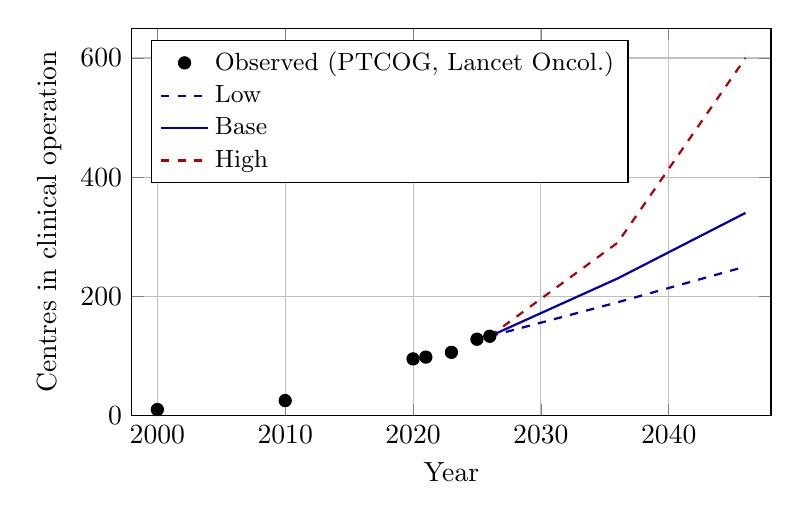
\begin{tikzpicture}
\begin{axis}[
  width=0.8\textwidth, height=6.5cm,
  xlabel={Year}, ylabel={Centres in clinical operation},
  xmin=1998, xmax=2048, ymin=0, ymax=650,
  grid=major, legend pos=north west, legend cell align=left,
  legend style={font=\small},
  xticklabel style={/pgf/number format/1000 sep=}
]
\addplot[only marks, mark=*, mark size=2.2pt, black] coordinates
  {(2000,10) (2010,25) (2020,95) (2021,98) (2023,106) (2025,128) (2026,133)};
\addlegendentry{Observed (PTCOG, Lancet Oncol.)}
\addplot[thick, blue!70!black, dashed] coordinates {(2026,133) (2036,190) (2046,250)};
\addlegendentry{Low}
\addplot[thick, blue!70!black] coordinates {(2026,133) (2036,230) (2046,340)};
\addlegendentry{Base}
\addplot[thick, red!70!black, dashed] coordinates {(2026,133) (2036,290) (2046,600)};
\addlegendentry{High}
\end{axis}
\end{tikzpicture}
\caption{Observed number of proton-therapy centres and the three projection
scenarios of Section~\ref{sec:scenarios}.}
\label{fig:growth}
\end{figure}

\section{The annual flow of new rooms}

The flow of new rooms is the quantity that determines the new-installation
market. IBA reports the number of rooms it sells and its share of new rooms sold,
from which the global figure follows (Table~\ref{tab:flow}). The IBA share
accounting excludes most Chinese domestic vendors (Shanghai APACTRON, Hefei
CIM, and others), which have received regulatory approval and are supplying
part of the Chinese pipeline, so the true global figure is probably 20--25 rooms
per year.

\begin{table}[h]
\centering
\caption{New proton-therapy rooms sold, from IBA investor reports \cite{iba_fy25,iba_h1_26}.}
\label{tab:flow}
\begin{tabular}{@{}lrrr@{}}
\toprule
Period & IBA rooms & IBA share of new rooms & Global rooms (implied) \\
\midrule
FY2024 & 4  & 56\% & $\approx 7$ \\
FY2025 & 12 & 63\% & $\approx 19$ \\
H1 2026 & 5 & 31\% & $\approx 16$ (half year) \\
\bottomrule
\end{tabular}
\end{table}

Two cross-checks give the same rate. The PTCOG construction list contains about
57 rooms opening over four years, and the planning list about 50 more, which
together with the Chinese domestic projects give a pipeline of 110--150 rooms
over five to seven years, i.e.\ 20--25 rooms per year. The IBA backlog alone,
46 sites in installation or production at roughly 1.5 rooms per site, is about
70 rooms. At its long-run share of 40--60\% this again implies a global pipeline
of 120--170 rooms.

The value of 19 rooms per year used in the ARGOS installation-market model
(file \path{costs/installation_market.csv}) is therefore a fair central
value, but it is the 2025 figure, which was IBA's second-best year ever. It
should be quoted as a range of 15--25 rooms per year.

\section{Demand ceiling}

The projection should be bounded by an estimate of how many patients could
plausibly be treated with protons. About half of all cancer patients require
radiotherapy. The fraction of radiotherapy patients who would benefit from
protons is debated: a survey of experts gave a median of 15\% (range 4--92\%),
while the fraction agreed by 95\% of respondents was 4.3\% \cite{bjr2022}.
Global cancer incidence is about 20 million new cases per year, rising to
30 million by 2040. The proton-eligible population is therefore of order
0.5--2 million patients per year.

Current capacity is far below this. With about 300 rooms treating 150--250
patients per room per year (exceptional single-device centres reach 1000), the
world treats roughly 40--60 thousand patients per year with protons, i.e.\
0.3--0.5\% of radiotherapy patients. Even the conservative 4\% eligibility would
require roughly ten times the present room count. Demand is not the constraint
in any of the scenarios below; system cost, reimbursement and the outcome of
the 35 ongoing phase~III trials comparing protons with photons are
\cite{iba_h1_26}.

A second, planning-based bound is the European Society for Radiotherapy and
Oncology rule of thumb of one proton centre per about 5 million inhabitants
\cite{estro2026}. Applied to the high-income world (1.3 billion people) this
gives about 260 centres; including upper-middle-income countries (about 4
billion) it gives about 800. The installed base would reach the first figure
in the 2040s under the base scenario and the second only under the high
scenario.

\section{Projection scenarios}
\label{sec:scenarios}

The three scenarios in Table~\ref{tab:scenarios} start from 133 centres and 310
rooms in 2026. All assume that new centres average 1.5--1.8 rooms and that
about one older room per year is retired.

\begin{description}
\item[Low.] Linear continuation of the 2020--2026 trend: 6 net new centres and
  14 net new rooms per year. This corresponds to reimbursement pressure in the
  United States and Europe, with only China sustaining growth.
\item[Base.] The current pipeline is built out and the flow rises modestly:
  20 rooms per year to 2030, 25 per year in 2031--2036, 30 per year thereafter.
  Centres grow at 8--10 per year. This is roughly 5\% annual growth of the room
  base early in the period, slowing to 3\% by the 2040s.
\item[High.] Sustained 8\% annual growth of the room base, a doubling every nine
  years, driven by China and India scaling to national coverage and by
  compact single-room systems reaching regional hospitals. This requires a
  step change in evidence or a large drop in system cost.
\end{description}

\begin{table}[h]
\centering
\caption{Projected proton-therapy installed base in clinical operation.}
\label{tab:scenarios}
\begin{tabular}{@{}lrrrrr@{}}
\toprule
 & \multicolumn{2}{c}{2036} & \multicolumn{2}{c}{2046} & New rooms \\
\cmidrule(lr){2-3}\cmidrule(lr){4-5}
Scenario & Centres & Rooms & Centres & Rooms & per year \\
\midrule
Low  & $\approx 190$ & $\approx 450$  & $\approx 250$ & $\approx 590$  & 14 \\
Base & $\approx 230$ & $\approx 550$  & $\approx 340$ & $\approx 850$  & 20--30 \\
High & $\approx 290$ & $\approx 670$  & $\approx 600$ & $\approx 1400$ & 25--60 \\
\bottomrule
\end{tabular}
\end{table}

Our informed guess is the base scenario: the installed base roughly doubles in
ten years and triples in twenty. Expressed as ranges, this is 200--250 centres
and 500--600 rooms in 2036, and 300--400 centres and 700--1000 rooms in 2046,
with a flow of 20--30 new rooms per year throughout.

\section{Consistency with revenue forecasts}

The market reports quoted in the funding deck put the systems market at about
\$1 billion in 2025 and forecast growth of 6--11\% per year to 2030--2035. At a
typical selling price of \EUR{}20--30 million per room including installation,
and allowing for service revenue on the installed base, a systems market of
\$1--1.5 billion corresponds to 20--35 rooms per year. The unit-based base
scenario is therefore consistent with the lower half of the analyst range, and
the high scenario with its upper half.

\section{Implications for the ARGOS market model}

\begin{enumerate}
\item \textbf{New-installation market.} The 19 rooms per year in the current
  model is a reasonable central value. A sensitivity range of 15--25 rooms per
  year should be shown, with 20--30 as the base expectation for the 2030s.
\item \textbf{Retrofit base.} The model assumes 300 eligible existing rooms,
  which equals today's entire installed base. If the retrofit window is the
  2030s, the eligible base is 450--550 rooms, so the assumption is conservative
  provided room compatibility holds.
\item \textbf{Recurring services.} The serviced base compounds with the
  installed base. Under the base scenario a product that captures a constant
  share of new rooms sees its service base grow by about 5\% per year from
  installations alone.
\item \textbf{Units.} Because new builds are mostly single-room, quoting the
  market in rooms rather than centres avoids overstating growth by roughly
  30\%.
\end{enumerate}

\section{Caveats}

The room count of the installed base is a trade estimate, not a PTCOG figure.
The PTCOG planning list is dated January 2025 and historically only 50--70\% of
planned projects are built on schedule. IBA share data exclude most Chinese
domestic vendors, so the Chinese contribution is the largest single uncertainty
in the flow. The demand ceiling depends on the proton-eligible fraction, which
spans an order of magnitude across experts. None of these uncertainties
changes the conclusion that the installed base will grow by a factor of two to
three over twenty years; they mainly affect the timing.

\begin{thebibliography}{99}

\bibitem{ptcog_map} Particle Therapy Co-Operative Group, \emph{Facilities world
map and facilities in clinical operation},
\url{https://ptcog.online/facilities-world-map/}, accessed September 2026.

\bibitem{ptcog_construction} Particle Therapy Co-Operative Group,
\emph{Facilities under construction}, list dated June 2026,
\url{https://ptcog.online/facilities-under-construction/}.

\bibitem{ptcog_planning} Particle Therapy Co-Operative Group,
\emph{Facilities in planning stage}, list dated January 2025,
\url{https://ptcog.online/facilities-in-planning-stage/}.

\bibitem{lancet2023} \emph{Global democratisation of proton radiotherapy},
Lancet Oncology 24 (2023),
\href{https://www.thelancet.com/journals/lanonc/article/PIIS1470-2045(23)00184-5/abstract}{doi:10.1016/S1470-2045(23)00184-5}.

\bibitem{frontiers2026} \emph{Advances in proton therapy technology and global
clinical applications}, Frontiers in Oncology (2026),
\url{https://pmc.ncbi.nlm.nih.gov/articles/PMC12932165/}.

\bibitem{iba_fy25} Ion Beam Applications, \emph{Full-year results 2025},
presentation of 27 March 2026, pp.~12--13,
\url{https://www.iba-worldwide.com/sites/default/files/2026-03/iba-fy25-results-presentation-en.pdf}.

\bibitem{iba_h1_26} Ion Beam Applications, \emph{Half-year 2026 results},
press release of 27 August 2026,
\href{https://www.iba-worldwide.com/iba-reports-half-year-2026-results-track-its-improved-profitability-trajectory}{iba-worldwide.com, ``IBA reports Half Year 2026 results''}.

\bibitem{iba_spain} Ion Beam Applications, \emph{IBA wins 10 proton therapy
system contract in Spain}, January 2023,
\url{https://www.iba-worldwide.com/iba-wins-10-proton-therapy-system-contract-spain}.

\bibitem{estro2026} ESTRO 2026 press release, \emph{Share proton therapy across
national borders and plan five new centres to maximise access for patients in
Europe}, \url{https://www.eurekalert.org/news-releases/1127623}.

\bibitem{bjr2022} \emph{Estimating the percentage of patients who might benefit
from proton beam therapy instead of X-ray radiotherapy}, British Journal of
Radiology 95 (2022) 20211175,
\url{https://pmc.ncbi.nlm.nih.gov/articles/PMC10993980/}.

\end{thebibliography}

\end{document}
